\newpage
\begin{flushright}
    \textbf{\Large{Ujian Tengah Semester}}
    \subsection*{Tahun 2023}
    \addcontentsline{toc}{subsection}{UTS - 2023}
\end{flushright}
\vspace{0.5cm}
\hrule height 2pt
\vspace{0.5cm}
\begin{center}
    \textbf{\large{MATERI}}
    \begin{enumerate}[leftmargin=*, label={\arabic*}.]
        \item Menyelesaikan pertidaksamaan yang melibatkan nilai mutlak.
        \item Mensketsa grafik fungsi.
        \item Menentukan range dan domain fungsi.
        \item Mencari nilai limit kiri dan nilai limit kanan fungsi.
        \item Mencari nilai limit fungsi di tak hingga.
        \item Menentukan kekontinuan fungsi pada suatu titik.
        \item Menyelesaikan masalah turunan implisit.
        \item Menyelesaikan permasalahan maksimum dan minimum.
    \end{enumerate}
\end{center}
\vspace{0.2cm}
\hrule height 1pt
\vspace{0.5cm}
\begin{center}
    \textbf{\large{SOAL}}
\end{center}
\begin{enumerate}[leftmargin=*, label={\arabic*}.]
\item Misalkan $\ds f(x) = \frac{\sqrt{5}\abs{x}}{x}$ dan $g(x) = -\sqrt{9-x^{2}}$.
\begin{enumerate}[label={\alph*}.]
    \item Tentukanlah domain dan range dari fungsi-fungsi tersebut!
    \item Tentukanlah himpunan penyelesaian dari: $f(x) \geq g(x)$.
\end{enumerate}
\item Diberikan fungsi $f$ dengan $f(x) = \floor{x}^2$.
\begin{enumerate}[label={\alph*}.]
    \item Sketsalah grafik fungsi $f$ tersebut!
    \item Tentukanlah
    \begin{enumerate}[label={\roman*}.]
        \item $f(-1)$
        \item $\ds\lim_{x\to -1^{+}} f(x)$
        \item $\ds\lim_{x\to -1^{-}} f(x)$
        \item $\ds\lim_{x\to -1} f(x)$
    \end{enumerate}
    \item Apakah fungsi $f$ kontinu di $x=-1$? Jelaskanlah!
    \item Jika $f$ tidak kontinu di $x=-1$, apakah ketidakkontinuan tersebut bisa 
    diperbaiki? Jelaskanlah!
\end{enumerate}
\item Carilah persamaan garis singgung dari kurva $(x^2+y^2)^2=(x-y)^2$ di titik $(1,-1)$.
\item Diketahui sebuah fungsi $f$ memenuhi \textbf{semua} kondisi berikut:
\begin{itemize}
    \item $f$ kontinu dimana-mana,
    \item $f(1)=2,f(2)=1,f(4)=4,f(6)=7,f(8)=3$,
    \item $f'(2)=0,f'(4)=1,f'(6)$ dan $f'(8)$ tidak ada,
    
    $f'(x)<0$ untuk $x < 2$ ataua $x>6$, $f'(x)>0$ untuk $2<x<6$,
    \item $f''(4) = 0$, $f''(x)<0$ untuk $4<x<6$ atau $x > 8$,
    
    $f''(x)>0$ untuk $x<4$ atau $6 < x < 8$.
\end{itemize}
\begin{enumerate}[label={\alph*}.]
    \item Di interval manakah fungsi tersebut naik atau turun, cekung ke atas atau 
    ke bawah? Apakah grafik fungsi tersebut mempunyai titik belok 
    (\textit{inflextion point})? Jelaskanlah!
    \item Tentukanlah titik-titik kritis dari fungsi $f$ pada interval 
    $\cintervalo*{1,\infty}$. Kemudian tentukanlah nilai maksimum dan minimum dari fungsi $f$ 
    pada interval tersebut (jika ada)!
    \item Buatlah sketsa grafik fungsi tersebut!
    \item Apakah terdapat bilangan $c$ dalam interval $\cintervalc*{1,6}$ yang memenuhi 
    Teorema Nilai Rata-rata untuk Turunan? Jelaskanlah! Jika ada, tentukanlah \textbf{semua} 
    bilangan $c$ tersebut.
\end{enumerate}
\item Seseorang $(A)$ berdiri di tepi sungai mengamati perahu yang melintas (seperti pada 
gambar di bawah). Asumsikan posisi perahu saat melaju selalu tepat di tengah sungai. Diketahui 
lebar sungai adalah $12$ meter. Jika sudut pengamatan antar $A$ dengan perahu adalah 
$\theta =\frac{\pi}{2}$rad dan kecepatan perubahan sudut $\theta$ adalah $3$rad/detik, berapa 
kecepatan perahu pada saat itu?
\vspace{0.2cm}
\begin{center}
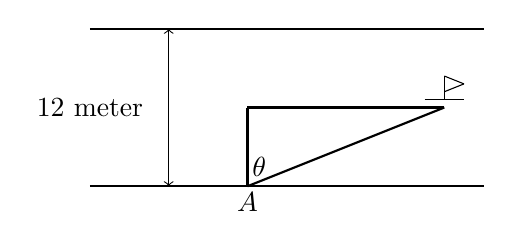
\begin{tikzpicture}
    \draw[thick] (-2,1)--(3,1);
    \draw[thick] (-2,-1)--(3,-1);
    \draw[thin, <->] (-1,-1)--(-1,1);
    \draw[thick] (0,-1)--(0,0);
    \draw[thick] (0,0)--(2.5,0);
    \draw[thick] (0,-1)--(2.5,0);
    \draw[thin] (2.25,0.1)--(2.75,0.1);
    \draw[thin] (2.5,0.1)--(2.5,0.4);
    \draw[thin] (2.75,0.3)--(2.5,0.4);
    \draw[thin] (2.75,0.3)--(2.5,0.2);
    
    \node at (-2,0) {$12$ meter};
    \node at (0.15,-0.75) {$\theta$};
    \node at (0,-1.2) {$A$};
    \end{tikzpicture}
\end{center}
\end{enumerate}
\vspace{0.2cm}
\hrule height 1pt
\vspace{0.5cm}
\begin{center}
    \textbf{\large{PEMBAHASAN}}
\end{center}
\begin{enumerate}[leftmargin=*, label={\arabic*}.]
\item Diberikan fungsi $\ds f(x) = \frac{\sqrt{5}\abs{x}}{x}$ dan $g(x) = -\sqrt{9-x^{2}}$.
\begin{enumerate}[label={\alph*}.]
    \item Pertama akan dicari domain dan range dari $f$.
    
    Untuk domainnya, karena $f$ memiliki bentuk rasional, maka penyebut tidak boleh nol. 
    Sehingga domain natural $f$ adalah bilangan real selain nol.\\
    Untuk rangenya, karena melibatkan bilangan mutlak $|x|$ dapat dilakukan pembagian 
    kasus untuk menghilangkan bentuk mutlaknya.\\
    Untuk $x>0$ maka
    \[
        \frac{\sqrt{5}\abs{x}}{x} = \frac{\sqrt{5}x}{x} = \sqrt{5}
    \]
    dan untuk $x < 0$ maka
    \[
        \frac{\sqrt{5}\abs{x}}{x} = \frac{\sqrt{5}(-x)}{x} = -\sqrt{5}
    \]
    sehingga range dari $f$ adalah $\sqrt{5}$ dan $-\sqrt{5}$.

    Diperoleh domain dari $f$ adalah $D_f=\set*{x\in \mathbb{R} \mid x\neq 0}$ dan 
    range $R_f=\set*{\sqrt{5},-\sqrt{5}}$

    Kedua akan dicari domain dan range dari $g$.

    Untuk domainnya, karena $g$ memiliki bentuk akar kuadrat, maka $9-x^{2}$ harus nonnegatif.\\
    Selesaikan pertidaksamaan berikut
    \[
        9-x^{2} \geq 0 \iff x^{2}-9 \leq 0 \iff (x+3)(x-3) \leq 0
    \]
    Maka titik stasionernya adalah $x=3$ dan $x=-3$.
    \begin{center}
    \begin{tikzpicture}
        \draw[stealth-stealth] (-5,0) node[below]{$-\infty$}--(5,0) node[below]{$\infty$};
        \draw (2,1) --(-2,1);
        \draw (-2,1)--(-2,-.1) node[below=0.2em]{$-3$};
        \draw (2,1)--(2,-.1) node[below=0.2em]{$3$};
                
        \node at (-3.5,.5) {$+$};
        \node at (0,.5) {$-$};
        \node at (3.5,.5) {$+$};
        \node [draw, shape = circle, fill = black, minimum size = 0.1cm, inner sep=0pt] at (2,0){};
        \node [draw, shape = circle, fill = black, minimum size = 0.1cm, inner sep=0pt] at (-2,0){};
        \end{tikzpicture}
    \end{center}
    Diperoleh domain dari $g$ adalah bilangan real $x$ dengan $-3 \leq x \leq 3$.

    Untuk range dari $g$, karena akar kuadrat selalu bernilai nonnegatif, maka kebalikannya selalu 
    nonpositif. Batas atas range fungsi $g$ adalah $0$. Untuk batas bawahnya akan dicari nilai minimum 
    dari $g$. Carilah titik stasioner $g$ pada domainnya.
    \begin{align*}
        g'(x) = 0 \iff &\drv{x}{-\sqrt{9-x^{2}}} = 0\\
        \iff &-\frac{1}{2}\frac{1}{\sqrt{9-x^{2}}}\drv{x}{9-x^{2}}=0\\
        \iff &\frac{x}{\sqrt{9-x^{2}}} = 0\\
        \iff & x=0
    \end{align*}
    Subtitusi $x=0$ ke $g$ diperoleh $g(0) = -\sqrt{9-0^{2}} = -\sqrt{9}=-3$. Ini adalah batas 
    bawah range $g$. Sehingga diperoleh range dari $g$ adalah $-3 \leq y \leq 0$.

    $\therefore$ Domain dan range dari $f$ adalah $D_f=\set*{x\in \mathbb{R} \mid x\neq 0}$ dan 
    $R_f=\set*{\sqrt{5},-\sqrt{5}}$ juga domain dan range dari $g$ adalah 
    $D_g=\set*{x\in \mathbb{R} \mid -3 \leq x \leq 3}$ dan 
    $R_g=\set*{y\in \mathbb{R} \mid -3 \leq x \leq 0}$.

\begin{center}
    \line(1,0){150}
\end{center}

    \item Akan dicari himpunan penyelesaian dari $\ds f(x) \geq g(x) 
    \iff \frac{\sqrt{5}\abs{x}}{x} \geq -\sqrt{9-x^{2}}$.

    Syarat dari kedua ruas mengharuskan nilai $x$ memenuhi kedua domain $f$ dan $g$. 
    Sehingga himpunannya penyelesaiannya hanya diantara $\cintervalc{-3,3} \cap x \neq 0$.
    Bagi kasus untuk menghilangkan bentuk nilai mutlak.

    \textbf{Kasus 1: $0 < x \leq 3$}\\
    Maka
    \begin{align*}
        \frac{\sqrt{5}\abs{x}}{x} \geq -\sqrt{9-x^{2}}
        \iff &\frac{\sqrt{5}x}{x} \geq -\sqrt{9-x^{2}} 
        &\text{definisi nilai mutlak} \\
        \iff &\sqrt{5} \geq -\sqrt{9-x^{2}}
        &\text{penyederhanaan}
    \end{align*}
    $\sqrt{5}>0$ dan $-\sqrt{9-x^{2}} \leq 0$, sehingga pertidaksamaan diatas selalu 
    bernilai benar. Sehingga pada kasus ini himpunan penyelesaiannya adalah $0 < x \leq 3$.

    \textbf{Kasus 2: $-3 \leq x < 0$}\\
    Maka
    \begin{align*}
        \frac{\sqrt{5}\abs{x}}{x} \geq -\sqrt{9-x^{2}}
        \iff &\frac{\sqrt{5}(-x)}{x} \geq -\sqrt{9-x^{2}} 
        &\text{definisi nilai mutlak} \\
        \iff &-\sqrt{5} \geq -\sqrt{9-x^{2}}
        &\text{penyederhanaan}\\
        \iff &\sqrt{5} \leq \sqrt{9-x^{2}}
        &\text{kedua ruas kalikan $-1$}\\
        \iff & 5 \leq 9-x^{2}
        &\text{kuadratkan kedua ruas}\\
        \iff &x^{2}-4 \leq 0
        &\text{kedua ruas jumlahkan $x^{2}-9$}\\
        \iff &(x+2)(x-2) \leq 0
    \end{align*}
    Maka titik stasionernya adalah $x=-2$ dan $x=2$.
    \begin{center}
        \begin{tikzpicture}
            \draw[stealth-stealth] (-5,0) node[below]{$-\infty$}--(5,0) node[below]{$\infty$};
            \draw (2,1) --(-2,1);
            \draw (-2,1)--(-2,-.1) node[below=0.2em]{$-2$};
            \draw (2,1)--(2,-.1) node[below=0.2em]{$2$};
                    
            \node at (-3.5,.5) {$+$};
            \node at (0,.5) {$-$};
            \node at (3.5,.5) {$+$};
            \node [draw, shape = circle, fill = black, minimum size = 0.1cm, inner sep=0pt] at (2,0){};
            \node [draw, shape = circle, fill = black, minimum size = 0.1cm, inner sep=0pt] at (-2,0){};
            \end{tikzpicture}
        \end{center}
    Pada kasus ini nilai $x$ yang memenuhi adalah $-2 \leq x \leq 2$. Iriskan dengan syarat 
    pada kasus ini diperoleh himpunan penyelesaiannya adalah $-2 \leq x < 0$.

    Gabungkan kedua kasus tersebut untuk memperoleh himpunannya penyelesaiannya \\
    $\set*{x \in \mathbb{R} \mid -2 \leq x < 0 \cup 0 < x \leq 3}$.

    $\therefore$ Diperoleh himpunan penyelesaian dari $\ds f(x) \geq g(x)$ adalah 
    $\set*{x \in \mathbb{R} \mid -2 \leq x < 0 \cup 0 < x \leq 3}$.
\begin{center}
    \line(1,0){300}
\end{center}
\end{enumerate}

\end{enumerate}

\begin{center}
    \line(1,0){300}
\end{center}